% % % % % % % % % % % % % % % % % % % % % % % % % % % % % % % % % % % % % % % %
% Formelsammlung von LaTeX4EI
%
% @encode: 	UTF-8, tabwidth = 4, newline = LF
% @author:	Emanuel Regnath
% @date:
%
% % % % % % % % % % % % % % % % % % % % % % % % % % % % % % % % % % % % % % % %

%---------------------------------------%
%			Regelungssysteme			%
%~~~~~~~~~~~~~~~~~~~~~~~~~~~~~~~~~~~~~~~%

% Document Class ===============================================================
\documentclass[fs, footer]{latex4ei}

\usepackage{mathtools}
\usepackage{tikz}
\usetikzlibrary{shapes,arrows}

% set imaginary unit to j
\renewcommand{\i}{\mathrm{j}}
% Fix "missing number, treated as zero" error for subsubsections
\titleformat{\subsubsection}{\normalsize\bfseries}{\thesubsubsection.\ }{0pt}{}



% DOCUMENT_BEGIN ===============================================================
\begin{document}

%\IfFileExists{git.id}{\input{git.id}}{}
%\ifdefined\GitRevision\mydate{\GitNiceDate\ (git \GitRevision)}\fi

% Split in 4 Columns ===========================================================
\begin{multicols*}{4}

% TITLE ========================================================================
\fstitle{Regelungssysteme}

% SECTION ======================================================================
%\section*{Allgemeines} % (fold)
% ==============================================================================
%\label{sec:allgemeines}
%	\symbolbox{
%		\begin{tabular}{rl}
%			$a_{\ir soll}$ & Sollwert \\
%			$a_{\ir ist}$ & Istwert \\
%			$a_{\ir d}$ & Abstandsfehler, Regelfehler
%		\end{tabular}
%	}

%\sectionbox{
%	\emph{Manuelle Steuerung}
%	Istwert wird nicht zum Ausgleich des Abstandsfehlers herangezogen

%	\emph{Manuelle Regelung}
%	$a_{\ir d}$ wird laufend erfasst und zur Korrektur herangezogen.
%}
% section allgemeines (end)



\section{Mathematische Grundlagen}

\sectionbox{


\subsection{Komplexe Zahlen $\cx z \in \C = \R^2$}
\pbox{3cm}{ 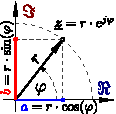
\includegraphics{./img/trigo.pdf} } \quad
\pbox{6cm}{
	$\cx z = \underset{\text{Karthesisch}}{a + b\i} = \underset{\text{Polarkoord.}}{r \cdot e^{\i \varphi}}$ \quad\ \boxed{ \underset{\text{Imaginäre Einheit}}{\i = \sqrt{-1}}}\\[0.4em]
	$\i^{2n} = -1^n$ \quad\ $\i^{2n+1} = -\i^n$ \quad\ $\i^{-1} = -\i$ \\[0.2em]
	Konjugiert: $\ol{\cx z} = a - b\i$ \\ $\cx z \ol{\cx z} = \abs{\cx z}^2 = a^2+b^2$\\[0.2em]
	$\cx z_1 \cdot \cx z_2 = r_1 \cdot r_2 \cdot e^{\i (\varphi_1 + \varphi_2)}$\\[0.2em]
	$z^{-1} = \frac{\ol{\cx z}}{\ol{\cx z} \cx z}=\frac{\ol{\cx z}}{a^2+b^2}$ }
}
\sectionbox{

\subsection{LaPlace - Korrespondenzen und Rechenregeln}

\tablebox{
	\begin{tabular*}{\columnwidth}{@{\extracolsep\fill}cc@{}}
	\ctrule
		$g(t)$ 														& 	$G(s) = \mathcal{L} \eset{g(t)}$	\\
		\cmrule
		Einheitsimpuls $\delta (t)$ 								&	$1$ 								\\
		Einheitssprung $\sigma (t)$									&	$\frac{1}{s}$ 						\\
		$t$															& 	$\frac{1}{s^2}$ 					\\
		$\frac{t^{n-1}}{(n-1)!}$ $(n = 1,2,3, \ldots)$				&	$\frac{1}{s^n}$ 					\\
		$t^n$				$(n = 1,2,3, \ldots)$					& 	$\frac{n!}{s^{n+1}}$ 				\\
		$e^{-at}$													&	$\frac{1}{s + a}$ 					\\
		$t e^{-at}$													&	$\frac{1}{(s + a)^2}$ 				\\
		$\frac{1}{(n-1)!} t^{n-1} e^{-at}$ $(n = 1,2,3, \ldots)$	& 	$\frac{1}{(s+a)^n}$ 				\\
		$t^n e^{-at}$		$(n = 1,2,3, \ldots)$					& 	$\frac{n!}{(s+a)^{n+1}}$ 			\\
		$\sin \omega t$												& 	$\frac{\omega}{s^2 + \omega^2}$		\\
		$\cos \omega t$ 											& 	$\frac{s}{s^2 + \omega^2}$ 			\\
		$\sinh \omega t$ 											& 	$\frac{\omega}{s^2 - \omega^2}$ 	\\
		$\cosh \omega t$ 											& 	$\frac{s}{s^2 - \omega^2}$ 			\\
		$\frac{1}{a} (1 - e^{-at})$									& 	$\frac{1}{s(s+a)}$					\\
		$\frac{1}{b-a} (e^{at} - e^{-bt}$							&	$\frac{1}{(s+a)(s+b)}$				\\
		$\frac{1}{b-a} (b e^{-bt}  - a e^{-at})$					&	$\frac{s}{(s+a)(s+b)}$ 				\\
		$\frac{1}{ab} (1 + \frac{1}{a-b} (b e^{-at} - a e^{-bt}))$	&	$\frac{1}{s(s+a) (s+b)}$			\\
 	\ctrule
	\end{tabular*}
}


\tablebox{
	\begin{tabular*}{\columnwidth}{@{\extracolsep\fill}ccc@{}}
	\ctrule
		Zeitbereich						& 	Frequenzbereich & Kommentar	\\
		\cmrule
		$c_1 g_1(t) + c_2 g_2 (t)$		&	$c_1 G_1 (s) + c_2 G_2 (s)$ & Linearitätsregel \\
		$g(t- T_t)$						&	 $e^{-sT_t} G(s)$ & Verschiebungsregel  \\
		$g(at)$							&	$\frac{1}{a} G(\frac{s}{a})$ & Ähnlichkeitsregel \\
		$e^{at}$						& $G(s-a)$		& Dämpfungsregel \\
		$\frac{\diff g}{\diff t}$	& $s G(s)$ & Differentiationsregel \\
		$\int \limits_0^t g(\tau) \diff \tau$ & $\frac{1}{s} G(s)$ & Integrationsregel \\
  	\ctrule
	\end{tabular*}
}
Hinweis: wird noch vervollständigt
}

\sectionbox{
\subsection{Exponentialfunktion und Logarithmus}
\begin{tabular*}{\columnwidth}{l@{\extracolsep\fill}ll}
	$a^x = e^{x \ln a}$ & $\log_a x = \frac{\ln x}{\ln a}$ & $\ln x \le x -1$\\
	$\ln(x^{a}) = a \ln(x)$ & $\ln(\frac{x}{a}) = \ln x - \ln a$ & $\log(1) = 0$\\
\end{tabular*}
}

\sectionbox{
\subsection{Matrizen}
	\subsubsection{$2 \times 2$-Matrix invertieren}
	$A^{-1} = \mat{a_{11} & a_{12} \\ a_{21} & a_{22}\\}^{-1} = \frac{1}{\det{A}} \mat{a_{22} & -a_{12} \\ -a_{21} & a_{11}\\}$
}

\columnbreak

% SECTION ====================================================================================
\section{Der Regelkreis}
% ============================================================================================
\sectionbox{
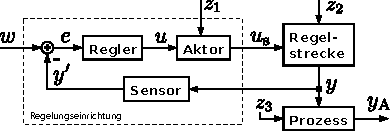
\includegraphics{./img/Regelkreis.pdf}

\tablebox{
	\begin{tabular*}{\columnwidth}{@{\extracolsep\fill}lll@{}} \ctrule
		Regelfehler & $e = w-y$ & Differenz zwischen „Soll“ und „Ist“\\
		Stellgröße & $u_{\ir S}$ & Eingang der Regelgröße\\
		Führungsgröße & $w$ & Sollverlauf, Vorgabe\\
		Aufgabengröße & $y_A$ & Die zu beinflussende Größe\\
		Regelgröße & $y$ & Die vom Sensor erfasste Größe\\
		Störgrößen & $z_i$ & Nicht beeinflussbare Störungen\\ \cbrule
	\end{tabular*} }

	\subsection{Standardübertragungsfunktionen}
	Gelten für den oben dargestellten Standardregelkreis.\\
	\emphbox{
		$G_0(s) = G_{\ir R} G_{\ir S} G_{\ir r}$\\
		$Y(s) = \frac{G_{\ir R} G_{\ir S}}{1 + G_0} W + \frac{G_{\ir S}}{1 + G_0} Z_1 + \frac{1}{1 + G_0} Z_2 + \frac{-G_0}{1 + G_0} Z_3$\\
		$E(s) = \frac{1}{1 + G_0} W + \frac{-G_{\ir S} G_{\ir r}}{1 + G_0} Z_1 + \frac{-G_{\ir r}}{1 + G_0} Z_2 + \frac{-G_{\ir r}}{1 + G_0} Z_3$
	}
}
Zustand: Ausgang eines Integrators

\section{Modellbildung, Linearisierung, lin. Systeme}
\sectionbox{\subsection{Zustandsbeschreibung linearer Systeme}


	mit $r$ Erregungen, $n$ Zustandsgrößen und $k$ Ausgängen.\\
	Die Zustandsgrößen $\vec x$ müssen einen stetigen Verlauf haben!

	\tablebox{
		\begin{tabular*}{\columnwidth}{@{\extracolsep\fill}ll@{}} \ctrule
			Allgemeine Zustandsgleichung: & $\bs{ \dot {\vec x}}(t) = \ma A \vec x(t) + \ma B \vec u(t) $\\
			Allgemeine Ausgangsgleichung: & $\vec y(t) = \ma C \vec x(t) + \ma D \vec u(t)$ \\ \cmrule
			Zustandsvariable & $\vec x(t) \in \mathbb R^n$ \\
			Ausgangsvariable & $\vec y(t) \in \mathbb R^k$ \\
			Erregungsvektor & $\vec u \in \mathbb R^r$ \\
			Systemmatrix & $\ma A\in \mathbb R^{n \times n}$ \\
			Einkopplungsmatrix & $\ma B \in \mathbb R^{n \times r}$ \\
			Auskopplungsmatrix & $\ma C \in \mathbb R^{k \times n}$ \\
			Durchgangsmatrix & $\ma D \in \mathbb R^{k \times r}$ \\
			\cbrule
		\end{tabular*}
	}

	Falls $\ma A, \ma B, \ma C$ oder $\ma D$ zeitvariabel sind handelt es sich um ein LTV-System, falls nicht um ein LTI-System.
}

\sectionbox{

	\subsection{Linearisierung}
	Gegegeben (nicht linear): \quad $\vec{\dot x} = \vec f(\vec x, \vec u)$ \qquad \quad $\vec y = \vec g(\vec x, \vec u)$
	\subsubsection{um eine allg. Referenzlösung}
	Referenzlösung $\vec x^*(t)$, $\vec y^*(t)$, $\vec u^*(t)$ mit $t \geq 0$ liegt vor. \\

	$\Delta \vec{\dot x} = \ma A(t) \Delta \vec x + \ma B(t) \Delta \vec u$\\
	$\ma A(t) = \left. \mat{\frac{\partial f_i}{\partial x_j}\\} \right|_{(\vec x^*(t),\vec u^*(t))}$ \quad
	$\ma B(t) = \left. \mat{\frac{\partial f_i}{\partial u_j}\\} \right|_{(\vec x^*(t),\vec u^*(t))}$\\ \\ \\
	$\Delta \vec y = \ma C(t) \Delta \vec x + \ma D(t) \Delta \vec u$\\
	$\ma C(t) = \left. \mat{\frac{\partial g_i}{\partial x_j}\\} \right|_{(\vec x^*(t),\vec u^*(t))}$ \quad
	$\ma D(t) = \left. \mat{\frac{\partial g_i}{\partial u_j}\\} \right|_{(\vec x^*(t),\vec u^*(t))}$\\

	\subsubsection{um eine Ruhelage}
	Spezielle Referenzlösung $\vec x^*$, $\vec y^*$, $\vec u^*$ konstant in Ruhelage.\\
	\begin{tabular}{ll}
	$\Delta \vec{\dot x} = \ma A \Delta \vec x + \ma B\Delta \vec u$ &  $\Delta \vec y = \ma C \Delta \vec x + \ma D\Delta \vec u$\\
	$\ma A = \left. \mat{\frac{\partial f_i}{\partial x_j}\\} \right|_{(\vec x^*,\vec u^*)}$ & $\ma C = \left. \mat{\frac{\partial g_i}{\partial x_j}\\} \right|_{(\vec x^*,\vec u^*)}$\\
	$\ma B = \left. \mat{\frac{\partial f_i}{\partial u_j}\\} \right|_{(\vec x^*,\vec u^*)}$ & $\ma D = \left. \mat{\frac{\partial g_i}{\partial u_j}\\} \right|_{(\vec x^*,\vec u^*)}$\\
	\end{tabular}
}


% ==============================================================================================
\section{Darstellung von LTI-SISO Systemen}
% ==============================================================================================

\sectionbox{
	\subsection{Differentialgleichungen (DGL)}
	Gleichung mit Funktion $y$ und deren $n$-ten Ableitungen $y',y'',...$\\
	Allgemeine DGL $n$-ter Ordnung:\\
	$\displaystyle a_n y^{(n)} + ... + a_1 y' + a_0 y = b_m x^{(m)} + ... + b_1 x' + b_0 x$\\
	Gesucht ist eine Funktion $y$ und keine Zahl! In der Praxis werden DGLs numerisch für diskrete Werte gelöst.


	\subsubsection{DGL-Systeme}
	Jede DGL lässt sich reduzieren auf ein DGL-System 1. Ordnung:\\
	1. Substituiere $x_i := y^{(i-1)}$ und drücke $\dot x_i$ durch $x_1,...,x_n$ aus.\\
	$\Ra$ \boxed{ \dot{\vec x}(t) = \ma A \vec x(t) + \vec s(t) } \quad mit $\vec x_{\ir ges} = \vec x_{\ir hom} + \vec x_{\ir part}$\\
	Hom. Lösung: 1. Bestimme EW $\lambda_i$ und Basis aus EV $\vec b_i$ von $\ma A$\\
	2. $\vec x_{\ir hom} = \vec c \cdot e^{(x-x_0)\ma A} = \sum\limits_{i = 0}^n c_i \cdot e^{\lambda_i x} \cdot \vec b_i$\\
	3. Bestimmung der Konstanten durch einsetzen der Anfangsbedingungen!\
}


\sectionbox{
	\subsection{Die Übertragungsfunktion}
	Beschreibt das System vollständig. Wird im Laplacebereich angegeben.\\
	Übertragungsfunktion einer lin. DGL $n$-ter Ordnung in Polynomform:\\
	\emphbox{ $\displaystyle G(s) = \frac{Y(s)}{U(s)} = \frac{\beta_m s^m + \ldots + \beta_1 s + \beta_0}{\alpha_n s^n + \ldots + \alpha_1 s + \alpha _0} = \frac{Z(s)}{N(s)}$ }
	($n =$ Ordnung der DGL $=$ Anzahl der Pole)\\
	\emphbox{Übertragungsfunktion der Zustandsbeschreibung: \\$\ma G (s) = \eset{\ma C (s \ma E - \ma A)^{-1} \ma B + \ma D}$} \\
	für $q = r = 1$ (SISO-System):
	$G(s) = \eset{ \vec c^{T} (s \ma E - \ma A)^{-1} \vec b + d}$\\
	\\
	Linearfaktorenform: $G(s) = \frac{\beta_m}{\alpha_n} \frac{\prod (s-z_j)}{\prod (s-p_i)}$\\
	Zeitkonstantenform: $G(s) = \frac{\beta_0}{\alpha_0} \frac{\prod (1+T_v s)}{\prod (1+T s)}$\\
	Partialbruchform: $G(s) = A_0 \sum \frac{A_j}{s-p_j} = A_0 + G^+(s)$\\
	%$H(\cx s) := \frac{Y(\cx s)}{X(\cx s)} = \frac{\sum b_k s^k}{\sum a_i s^i}= k \frac{\prod (s-z_k)}{\prod (s-p_i)}$ \qquad $k = \frac{b_m}{a_n}$\\

	\subsubsection{Dominierendes Verhalten und Ordnungsreduktion}
	Pole nahe der Imaginärachse dominieren. Anwendung auf \emph{Zeitkonstantenform}.
	\begin{itemize}
		\item Sortiere Zeitkonstanten nach Größe
		\item Gilt zwischen 2 benachbarten Werten $T_i > 10 \tau_j$, so können $\tau_j$ und alle kleineren Werte vernachlässigt werden.
		\item $G(s) = \frac{K}{\prod\limits_{i}{(1 + T_i s)}} \frac{1}{\prod\limits_{j}{(1 + \tau_j s)}} \rightarrow G^*(s) = \frac{K}{\prod\limits_{i}{(1 + T_i s)}}$
	\end{itemize}
	Hinweise:
	\begin{itemize}
		\item Zeitkonstanten aus Polen: $T_i = \frac{1}{\abs{p_i}}$
		\item Pole auf oder rechts von Imaginärachse dürfen \emph{nicht} vernachlässigt werden.
	\end{itemize}

	\subsubsection{Wichtige spezielle Übertragungsfunktionen (Frequenzantw.)}
	\begin{tabular}{@{}ll|ll}
		$u(t)$ & $U(s)$ & Zeitantwort & Frequenzantwort\\ \mrule
		$\delta(t)$ & $1$ & Gewichtsfunktion $g(t)$ & $G(s)$\\
		$\sigma(t)$ & $\frac{1}{s}$ & Übergangsfunktion $h(t)$ & $H(s)$\\
		$t \cdot \sigma(t)$ & $\frac{1}{s^2}$ & Anstiegsantw. & Rampenantwort\\
		%$e^{\i \omega}$ & & Frequenzgang $H(\i \omega)$\\
	\end{tabular}\\


	ÜTF Regler $G_{\ir R}(s)$\\
	ÜTF Steller/Strecke $G_{\ir S}(s)$\\
	ÜTF Rückführung $G_{\ir r}(s)$\\
	ÜTF offener Regelkreis $G_{\ir O}(s) = G_{\ir R}(s) G_{\ir S}(s) G_{\ir r}(s)$\\
	Führungsübertragungsfunktion $G_w(s) = \frac{Y(s)}{W(s)}$\\
	Störübetragungsfunktion $G_z(s) = \frac{Y(s)}{Z(s)}$\\

	Es gilt $N_{\ir RK}(s) = N_{\ir O} + Z_{\ir O}$

	\subsubsection{Frequenzgang}
	Der FG ist die Systemantwort bei harmonischer Erregung $u(t) = e^{\i \omega t}$\\
	Nach dem Einschwingen (wird ignoriert) ist die Systemantwort ebenfalls harmonisch, allerdings mit anderer Amplitude und Phase.\\
	Frequenzgang: $G(\i \omega) = G(s)|_{s = 0 + \i \omega, \omega > 0} = A(\omega) e^{\i \varphi(\omega)}$
}


\sectionbox{
	\subsubsection{Zustandsraummodell}
	DGL $n$-ter Ordnung:\\ $a_n y^{(n)} + ... + a_1 y' + a_0 y = b_m u^{(m)} + ... + b_1 u' + b_0 u$\\
	Lässt sich immer reduzieren auf ein DGL-System 1. Ordnung:\\
	$\vec{\dot x} = \mat{0 & 1 & 0 & \ldots & 0 \\ 0 & 0 & 1 & \ldots & 0 \\ \ldots & \ldots & \ldots & \ldots & \ldots \\ 0 & 0 & 0 & \ldots & 1 \\ -a_0 & -a_1 & -a_2 & \ldots & -a_{n-1} }\vec{x} + \mat{0 \\ \vdots \\0 \\ 1} u$ \\
	wobei $\vec{x} = \frac{1}{b_0}\mat{y & y' & \cdots & y^{(n)}}^{\top}$

\textbf{Normalformen} \\
\begin{itemize}
	\item Kanonische Normalform \\
		zur Entkopplung des Systems bzw. der zugehörigen DGLs.

		Wähle $\ma T$, sodass $\ma T^{-1} \ma A \ma T$ eine Diagonalmatrix ist:

		$\ma T^{-1} \ma A \ma T = \diag ( \lambda_i)$

		${\vec{\dot x_k}} = \diag (\lambda_i) \vec x_k + \vec b_k u$

		$y = \vec{c_{k}^{T}} \vec{ x_{k}} + d u$

		% ??? $G(s) = \sum \frac{A_k}{s - p_k}$
	\item Regelungsnormalform: \\
		nur die letzte Zustandsvariable $x_{Rn}$ wird direkt durch den Eingang beeinflusst

		Steuerbarkeitsmatrix: $\ma S_S = \mat{\vec b & \ma A \vec b & \ma A^2 \vec b & \ldots & \ma A^{n-1} \vec b}$

		! RNF existiert nur falls $\ma S_S$ regulär ist $\ra $ System ist vollst. steuerbar

		Transformationsmatrix $\ma T_R = \mat{ \vec s_R^T \\ \vec s_R^T \ma A \\ \vec s_R^T \ma A^2 \\ \vdots \\ \vec s_R^T \ma A^{n-1}}^{-1}$

	\item Beobachtungsnormalform: \\
		$\dot{\vec x }_B = \ma A_B \vec x_B + \vec b_B u$  \quad $\vec x_B (t_0) = \vec x_{B0}$

		$y = \vec c_B^T \vec x_B + d u$

		Beobachtbarkeitsmatrix

		$\ma S_B = \mat{ \vec c^T & \vec c^T \ma A & \vec c^T \ma A^2 & \ldots & \vec c^T \ma A^{n-1} }^{\top}$

		Transformationsmatrix

		$\ma T_B = \mat{ \vec s_B & \ma A \vec s_B & \ldots & \ma A^{n-1} \vec s_b}$

		$\ma A_R = \ma A_B^T$ \quad $\vec b_R = \vec c_B$ \quad $\vec c_R = \vec b_B$
	\end{itemize}

}
\sectionbox{
	\subsection{Schockschaltbildalgebra}
	\textbf{Serienschaltung:} $G(s) = \prod G_i(s)$\\
	\textbf{Parallelschaltung:} $G(s) = \sum G_i(s)$\\
	\textbf{Kreisstruktur:} $G(s) = \frac{G_{\ir Vor}(s)}{1 \mp G_{\ir Vor}(s) G_{\text{Rück}}(s)}$\\
	Umformung: $\frac{\frac{A}{B}}{1 \pm \frac{A}{B} \frac{C}{D}} = \frac{DA}{AC \pm BD}$ \qquad\qquad $\frac{1}{1 + \frac{A}{B}} = \frac{B}{A+B}$\\
	Umformung bei $G_{\text{Rück}} = 1$: $\frac{\frac{A}{B}}{1 \pm \frac{A}{B}} = \frac{A}{A \pm B}$\\

	\pbox{4cm}{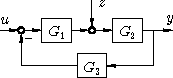
\includegraphics{./img/control_circle.pdf}} \quad \pbox{4cm}{$G_S = \frac{Y}{U} = \frac{G_1 G_2}{1 + G_1 G_2 G_3}$ \\[1em] $G_Z = \frac{Y}{Z} = \frac{G_2}{1 + G_2 G_3 G_1}$ }

}


\sectionbox{
	\subsection{Anfangs und Endwertsatz}
	Vorraussetzung: höchstens ein einfacher Pol von $Y(s)$ am Ursprung, die restlichen in der linken Halbebene.\\

	\emphbox{ $\lim\limits_{\mathclap{\phantom{:} t \ra 0^+}} \; x(t) = \lim\limits_{\strut \mathclap{s \ra \infty}} \; s X(s)$ \qquad\qquad $\lim\limits_{\strut \mathclap{t \ra \infty}} \; x(t) = \lim\limits_{\mathclap{\phantom{:} s \ra 0^+}} \; s X(s)$ } \\

	Anfangswertsatz: $y(t = 0^+)  = \lim\limits_{s \ra \infty} [s G(s)U(s) ]$\\
	Endwertsatz: $y(t \ra \infty) = \lim\limits_{s \ra 0} [s G(s)U(s) ]$\\
	Regelfehler: $e(\infty) = w(\infty) - y(\infty)$ = $\lim\limits_{\mathclap{s \ra 0}} s \Big(1- G_w(s)\Big) W(s)$
}



\section{Systembausteine}
\sectionbox{

\tablebox{
	\begin{tabular*}{\columnwidth}{@{\extracolsep\fill}lll@{}}
	\ctrule
	System & Zeitbereich & Frequenzbereich $G(s)$ \\
	\cmrule
	P-System 		& $y(t) = K_{\ir P} u(t)$ 								& $K_{\ir P}$ \\
	I-System 		& 	$\dot y(t) = K_{\ir I} u(t)$ 						& $\frac{K_{\ir I}}{s}$ \\
	D-System 		& 	$y(t) = K_{\ir D} \dot u(t)$ 						& $K_{\ir D} s$ \\
	Totzeitsystem 	& 	$y(t) = K u(t-T_t)$									& $K e^{-s T_t}$ \\
	PT$_1$-Systeme 	& 	$T \dot y(t) + y(t) = K_{\ir P} u(t)$ 				& $\frac{K_{\ir P}}{1 +sT}$\\
	PT$_2$-Systeme 	& 	$\ddot y(t) + 2D\omega_0 \dot y(t) + \omega_0^2 y$ 	& $K_{\ir P} \frac{\omega_0^2}{s^2 + 2D\omega_0 s+ \omega_0^2}$ \\
					&	$= K_{\ir P} \omega_0^2 u(t)$\\
	\cbrule
	\end{tabular*}
}


	Einstellzeit $T_{\ir Ein}$ bis Signal im 5\% Bereich stabil.

% Tutoremail: artur.lohrer@gmx.de
% Turium:
% u* 1/(s^2+s a_0) +



% Prüfung: Stab–Waagen Versuch Jacobimatrizen ausrechen!
% Passwort Moodle: rs1-2013


Übung:\\
1. Verschieben der Summationsstelle\\
2. Vertauschen/Zusammenfassen der Summationsstelle\\

\subsection{PT$_2$ Systeme}
DGL: $\ddot y + 2D \omega_0 \dot y + \omega_0^2 y = K \omega_0^2 u$

Übertragungsfunktion: $G(s) = K \frac{\omega_0^2}{s^2 + 2 D \omega_0 s + \omega_0^2}$

$n$ Pole $\ne 0$ im Nenner: T$_n$ System\\
Allgemeine Polform: $p_{1/2} = \underbrace{-\omega_0 D}_{\sigma_e} \pm \i \underbrace{\omega_0 \sqrt{1 - D^2}}_{\omega_e}$\\

\begin{tabular}{@{}p{1cm}l}
Dämpfung & Systemverhalten\\ \mrule
$D < 0$ & System instabil\\
$D = 0$ & Grenzstabil, Dauerschwingung, Resonanzkatastrophe\\[0.5em]
\parbox{1cm}{$D \in ]0;1[$ \vspace{0.7cm}} & \parbox{5cm}{Abkl. Schwingung, Konjugiert komplexe Pole\\
	Für $0 < D < \frac{\sqrt{2}}{2}$ Resonanz $\omega_r = \omega_0 \sqrt{1-2D^2}$\\
	$A_{\ir max} = A(\omega_r) = \frac{K}{2D\sqrt{1-D^2}}$ }\\
$D = \frac{\sqrt{2}}{2}$ & \emph{Minimale Einschwingzeit $T_{\ir Ein}$}\\
$D = 1$ & Aperiodisch $\leftrightarrow$ reeler Doppelpol $\leftrightarrow$ Diskriminante = 0\\
$D > 1$ & Griechfall, verschiedene reele Pole\\
\end{tabular}
}




% SECTION ======================================================================
\section{Stabilität von LTI-Systemen}
% ==============================================================================
\sectionbox{
\subsection{Definitionen}
\textbf{stabil bzw. zustandsstabil:} $\norm{ \vec x_0 } < \varepsilon_1 \Ra \norm{ \vec x(t) } < \varepsilon_2$

\textbf{asymptotisch stabil:} zustandsstabil und $\lim\limits_{t \ra \infty} \norm{\vec x(t)} = 0$

\textbf{robust stabil:} bleibt auch bei Paramterabweichungen stabil.

Beispiel untersch. Systemmatrix: $\forall \ma A \in \eset{\ma A_{\min}; \ma A_{\max}}$ stabil
}

\sectionbox{
\subsubsection{Stabilitätsbedinung für LTI-Systeme}
\emphbox{$\Re{\lambda_i (A)} < 0 \quad i = 1, \ldots, n$}
}

\sectionbox{
\subsection{Routh-Hurwitz-Kriterium}

	\textbf{Gegeben:}

	charakteristisches Polynom:
	$N(s) = b_n s^n + b_{n-1} s^{n-1} + \ldots + b_0$ \\

	\textbf{Notwendige Bedingung:}
	$b_i > 0 \quad \forall i \le n$ oder $b_i < 0 \quad \forall i \le n$


	Betrachte Koeffizienten $b_i$ des Nenners von $G(s)$\\
	\begin{tabular}{ll}
	$n = 1:$ & $b_1 > 0,\quad b_0 > 0$\\
	$n = 2:$ & $b_2 >0,\quad b_1 > 0,\quad b_0 > 0$\\
	$n = 3:$ & $b_3 > 0,\quad b_2 > 0,\quad b_1 > 0,\quad b_0 > 0$\\
			 & $b_2 b_1 - b_0 b_3 > 0$\\
	$n = 4:$ & $b_4 > 0,\quad b_3 > 0, \quad b_2 > 0, \quad b_1 > 0,\quad b_0 > 0$\\
			 & $b_3 b_2 b_1 - b_0 b_3^2 - b_1^2 b_4 > 0$\\
	\end{tabular}
	\\ \\
	\emphbox{
	Ein System ist dann und nur dann stabil, wenn gilt:

	$b_n > 0$ und  alle $n$ Hurwitzdeterminanten $> 0$
	}

}
\sectionbox{
\subsection{Direkte Methode von Lyapunov}
    Der GGP $\vec{x}^*$ ist asymptotisch stabil, wenn eine Lyapunov-Funktion $V(\vec{x})$ gefunden werden kann mit:
    \begin{enumerate}
    	\item $V(\vec{x}^*)=0$
    	\item $V(\vec{x})>0\quad\forall \vec{x}$
	    \item $\frac{\diff}{\diff t} V(\vec{x})<0 \quad \forall \text{ Lösungen } \vec{x}(t) \text{ der DGL}$


    \end{enumerate}
	Für lineare System mit Systemmatrix $\ma A$: \qquad \boxed{ \ma A^\top \ma P + \ma P \ma A = - \ma Q }\\

	\cookbox{Direkte Methode von Lyapunov für lineare Systeme}{
		\item Wähle $\ma Q \ = \ma E_n$
		\item Berechne $\ma P$
		\item 	System asymptotisch stabil $\Longleftrightarrow$ $\ma P$ symm. und pos. definit
	}

}

\sectionbox{
\subsection{Eigenwerte und Polstellen}
%Systemmatrix $\ma A$: Alle EW $\lambda_i < 0$\\

	\subsubsection{Pole}
	Pole $p_i$ von $G(s)$: Alle $\Re{p_i} < 0$\\
	$G(s) = \sum \frac{k_i}{s-p_i}$ \qquad $\Ra \quad g(t) = \sum k_i e^{p_i t}$

	\subsubsection{Dominanz im System}
	Vorraussetzung $T_{\max} > \tau_{\min}$\\
	Große Zeitkonstanten, Pole mit pos. Realteil (instabil)
}

\sectionbox{
\subsection{Zustandssteuerbarkeit und -beobachtbarkeit}

	\subsubsection{Zustandssteuerbarkeit}
		Def.: Man kann mit $\vec u(t)$ in endlicher Zeit $\vec x(t < \infty) = 0$ erreichen\\\\
		Bedingung: $\mathrm {Rang}(\ma Q_{SZ})=n$ bzw. $\det(\ma Q_{SZ})\ne 0$ \\
		mit Zustandssteuerbarkeitsmatrix $\ma Q_{SZ}=[\ma B, \ma A \ma B, \ldots, \ma A^{n-1} \ma B]$

	\subsubsection{Zustandsbeobachtbarkeit}
		Def.: Anfangszustände $\vec x_0$ aus Verlauf $\vec y(t < \infty)$ bestimmbar \\\\
		Bedingung: $\mathrm {Rang}(\ma Q_{BZ})=n$ bzw.  $\det(\ma Q_{BZ})\ne 0$ \\
		mit Zustandssteuebeobachtbarkeitsmatrix \\ $\ma Q_{SZ} = [\ma C^\top, \ma A^\top \ma C^\top, \ldots, (\ma A^\top)^{n-1} (\ma C^\top)]$
}

\sectionbox{
\subsection{E/A (BIBO) Stabilität (äußere Stabilität)}

\emphbox{
$\Re{p_i} < 0 \quad i = 1,2, \ldots n$
} \\

$\sum$ ist E/A-stabil, falls gilt:

\textbf{Definition:}
$\norm{ \vec u(t) } < \varepsilon_1 \Ra \norm{ \vec x(t) } < \varepsilon_2$ \\

\textbf{Pole der Übertragungsfunktion}:

$\Re{p_i} < 0 \quad i = 1,2, \ldots n$ \\

Stabilität anhand von PN-Diagramm und Impulsantwort:\\ \\
\setlength{\tabcolsep}{1mm}
\begin{tabular}{@{\extracolsep\fill}cccccc@{}}
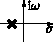
\includegraphics{./img/blocks/PN_1.pdf} & 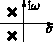
\includegraphics{./img/blocks/PN_2.pdf} & 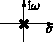
\includegraphics{./img/blocks/PN_3.pdf} & 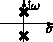
\includegraphics{./img/blocks/PN_4.pdf} & 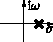
\includegraphics{./img/blocks/PN_5.pdf} & 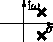
\includegraphics{./img/blocks/PN_6.pdf} \\
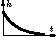
\includegraphics{./img/blocks/PN_1h.pdf} & 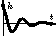
\includegraphics{./img/blocks/PN_2h.pdf} & 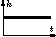
\includegraphics{./img/blocks/PN_3h.pdf} & 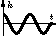
\includegraphics{./img/blocks/PN_4h.pdf} & 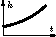
\includegraphics{./img/blocks/PN_5h.pdf} & 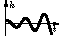
\includegraphics{./img/blocks/PN_6h.pdf} \\
stabil & stabil & stabil$^*$. & stabil$^*$ & instabil & instabil\\
\end{tabular}\\
$^*$: An der Stabilitätsgrenze.\\

\subsubsection*{Zusammenhang zwischen innerer und äußerer Stabilität}
Falls $\sum$ vollst. steuer- und beobachtbar, oder nur auf einer Untermenge steuer- und beobachtbar:
$\Ra$ asymptotisch stabil $\Leftrightarrow$ E/A-stabil\\

\subsubsection*{Stabilitätsreserve}
Absolut: $\sigma_{gr} = \min p_i$ \\

Relativ: $D_{gr} = \cos(\varphi_{gr})$
}

\columnbreak
% SECTION ======================================================================
\section{Stabilitätsanalyse im Frequenzteich}
% ==============================================================================
für alle Systeme (auch mit Totzeit) möglich.

\symbolbox{
\begin{tabular}{cc}
	$\omega_A$ & Abtastfrequenz \\
	$\omega_g$ & Grenzfrequenz \\
	$\omega_B$ & Systembandbreite
\end{tabular}
}


\sectionbox{
\subsection{Frequenzgangfunktion  $G(\j \omega)$}
Beschreibt die Auswirkungen von sinusförmigen Anregungen auf die Systemantwort.

Die Auswirkungen auf Amplitude $A$ und Phasenverschiebung $\varphi$ ergeben die Frequenzgangfunktion $G(\j \omega)$

	\emphbox{$G(\j \omega) = A(\omega) e^{\j \varphi (\omega)} = \Re {G(\j \omega)} + \j \Im{G(\j \omega)}$ }
	\pbox{4cm}{ 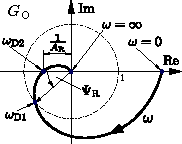
\includegraphics{./img/OK_GO.pdf} } \quad
	\pbox{4cm}{
		\emph{Einschwingzeit:} $T_{\ir Ein} \approx \frac{3}{\omega_{\ir D1}}$\\
		\\
		Stabilitätskriterien mit Totzeit:\\
		geschl. RK ist E/A \textbf{stabil} falls:\\
		Phasenrand $\Psi_{\ir R} > 0$, bzw.\\
		Amplitudenrand $A_{\ir R} > 1$\\
		\\
		$\Psi_{\ir R} \approx 30^\circ \Leftrightarrow $ gutes Störverhalten\\
		$\Psi_{\ir R} \approx 60^\circ \Leftrightarrow $ gutes Folgeverhalten
	}

	\begin{tabular}{@{}ll@{}}
	\textbf{Kenngrößen:} & Bodediagramm:\\ \mrule
		Amplituden-Durchtrittsfrequenz $\omega_{D1}$: & $A(\omega_{D1}) = 1$\\
		Phasen-Durchtrittsfrequenz $\omega_{D2}$ & $\varphi (\omega_{D2}) = - \pi = -180^\circ$\\
		Phasenrand/Phasenreserve $\Psi_R$: & $\Psi_R = \varphi (\omega_{D1}) + \pi$\\
		Amplitudenrand/-reserve $A_R$ $(= K_{\ir krit})$ & $\frac{1}{A_R} = A (\omega_{D2})$
	\end{tabular}
}

\sectionbox{
	\subsubsection{Schwingbedingung}
	Situation in der der Regelkreis sich selbst erregen und (theoretisch) mit $\omega_{\ir krit}$  weiterschwingen würde.\\

	\emphbox{$G_0 (\j \omega) \overset{!}{=} -1 + \i 0$} \\

	Der Regelkreis befindet sich an der Stabilitätsgrenze:

	$\Ra$ Dauerschwingungen mit $\omega = \omega_{\ir krit}$ und $K = K_{\ir krit}$ (krit. Verstärkung)
}

\sectionbox{
	\subsection{Nyquist}
	\subsubsection{Nyquist Ortskurve}

	Die Nyquist Ortskurve ist die Frequenzgangortskurve des offenen Regelkreises $G_o (s)$

	\subsubsection{Nyquist Kriterium}

	Ein geschlossener linearer Regelkreis ist dann stabil, wenn die Ortskurve des offenen Regelkreises $G_0(\i \omega)$
	\begin{enumerate}
		\item \emph{nicht} durch $-1 + 0\i$ verläuft und
		\item die Phasenänderung von $-1 + 0\i$ aus gesehen folgende Bedingung erfüllt
	\end{enumerate}
	\emphbox{$W_{\ir ist} = \mathop{\Delta}\limits_{\omega = 0}^{\omega = \infty} \Phi \stackrel{!}{=} W_{\ir soll} = \pi n_{\ir rechts} + \frac{\pi}{2} n_{\ir auf}$}\\
	$n_{\ir rechts}$: Anzahl der Pole von $G_0(s)$ rechts der Imaginärachse\\
	$n_{\ir auf}$: Anzahl der Pole von $G_0(s)$ auf der Imaginärachse
}

\sectionbox{
	\subsubsection{Linke-Hand-Regel}
	anwendbar falls $n_r = 0$ und $n_a \le 1$ \\

	\textbf{Definition:}

	Der geschlossens Regelkreis ist stabil, wenn beim Entlangwanderen auf der $G_0 (\j \omega)$- Ortskurve von $\omega = 0 $ nach $\omega = \infty$ (Blick nach vorne! ) der kritische Punkt $P_{\ir krit}$ beim Passieren des diem am nächsten liegenden Ortskurvenabschnittes stets linker Hand liegt.
}

\sectionbox{
	\subsection{Bode-Diagramm}
	aufteilung der Frequenzgangfunktion in Phase ($\varphi (\omega)$) und Amplitude ($A ( \omega)$).

	\emphbox{$G (\j \omega) = A(\omega) e^{\j \varphi (\omega)}$}

	\subsubsection{Typische Regelstrecken}

	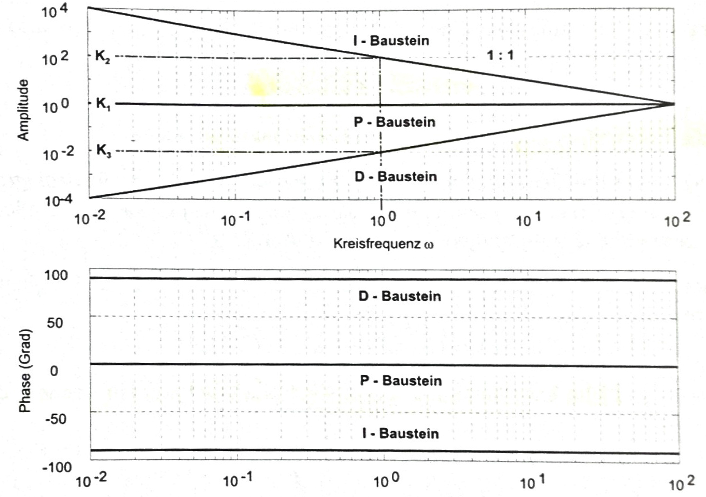
\includegraphics[width=\columnwidth]{img/Bode-Diagramme_Regler.pdf}

	Die Eckfrequenz $\omega_E$ bezeichnet die Stelle von $G(j\omega)$ mit $A(\omega)=\frac{K}{\sqrt{2}}$

	Zusätzlich gilt: $\omega_E = \frac 1 T$

	Im $PT_1$-System gilt:
	$A (\omega_E) = \frac{K}{\sqrt 2}$ \quad $\omega_B = \omega_E$

	\tablebox{
		\begin{tabular*}{\columnwidth}{@{\extracolsep\fill}lll@{}}
		\ctrule
			Baustein & Auswirkung auf Amplitude & Ausw. Phase \\ \cmrule
			Verstärkung $K$ & $A(w) = K$ & $\varphi (\omega) = 0$ \\
			Pol im Ursprung & 1:1 Abfall, $A(\omega=1)=1$& $\varphi ( \omega ) = -90^\circ$ \\
			Reeller Pol $s=-\omega_E$ \hspace{-1em} & $A(\omega) = 1$ für $\omega \ll \omega_E$ & $\varphi(\omega) = 0$\\
			& 1:1 Abfall für $\omega \gg \omega_E$ & $\varphi(\omega) = -90^\circ$ \\
		\ctrule
		\end{tabular*}
	}
	Weitere Auswirkungen siehe Skript S. 130
}

\sectionbox{
	\subsection{Systeme mit Totzeit}
	lassen sich schwer regeln.\\

	Stabilitätsbedingung: $0 < K_0 < 1$

	bleibende Regeldiffernz nach Sprunganregung $\sigma (t)$ immer $ > 0,5$
}




% SECTION ======================================================================
\section{Grundlagen Reglerentwurf}
% ==============================================================================
Ziel: ideale Führung und ideal Störungsrobust:\\
$y(t) \stackrel{!}{=} 1 \cdot w(t) + \sum 0 \cdot z_i(t)$\\
Generell: P-Strecke mit I-Regler, I-Strecke mit P-Regler!

\sectionbox{
	\subsection{Entwurfsvorschriften}
	Stabilität: $\Psi_R > 0$

	Gutes stationäres Verhalten: $\abs{G_o (j \omega)}_{\omega \ll \omega_D1} \gg 1$
	$\ra$ I-Regler oder starker P-Regler

	Gutes Einschwingverhalten:

	$\abs{G_o (\j \omega)} \approx \frac{1}{\frac{\omega}{\omega_{D1}}}, \quad 0,5 \omega_{D1} \le \omega \le 5 \omega_{D1}$

	Bandbreite: $\omega_B \approx \omega_{D1}$

	Einschwingzeit: $T_{\ir ein} = 3 \tilde{T} \approx \frac{3}{\omega_{D1} }$

	gutes Folgeverhalten: $\Psi \approx 60^\circ$

	gutes Störverhalten: $\Psi \approx 30^\circ$

	wenig Messrauschen: $\left. \abs{G_o (\j \omega)}\right|_{\omega \gg \omega_{D1}} \ll 1$
}

\sectionbox{
	\subsection{Reglerentwurf nach Ziegler-Nichols}
	\begin{tabular}{llll}
		Regeltyp & $K_R$ & $T_n$ & $T_v$\\ \mrule
		P & 0.5 $K_{R, \ir krit}$ & $(\infty)$ & (0)\\
		PI & 0.45 $K_{R, \ir krit}$ & 0.85 $T_{\ir krit}$ & (0)\\
		PID & 0.7 $K_{R, \ir krit}$ & 0.4 $T_{\ir krit}$ & 0.15 $T_{\ir krit}$\\
	\end{tabular}
}

\sectionbox{
	\subsection{Wurzel Ortskurven WOK}
	\pbox{4cm}{
		Entspricht Verlauf der Polstellen $p^{\ir RK}$ des geregelten Kreises $G_{\ir RK}$ für steigendes $K$\\[1em]
		WOK ist immer symm. zur Realachse!\\[1em]
		Totzeitglied im System $\Ra$ WOK ungültig!\\
	} \quad
	\pbox{3cm}{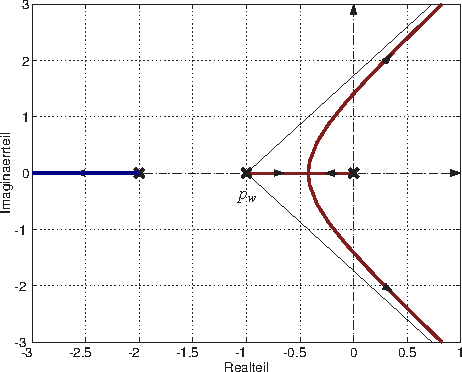
\includegraphics[width = 2.5cm]{./img/wok.pdf}}

	\emphbox{$G_0 (s; K) = K \frac{Z_0 (s)}{N_0 (s) } = KQ \frac{\prod_{\mu = 1}^{m} (s-q_\mu^0)}{\prod_{\nu = 1}^n (s-p_\nu^0)}$}
	\\ \\

	Falls offener RK $G_0$ linear vom Faktor $K$ abhängt gelten folgende Regeln für den \emph{geschlossenen} RK $G_{\ir RK}$:
	\begin{itemize}
		\item Die Pole $p^{\ir RK}$ liegen symm. zur reellen Achse bzw. darauf
		\item $n$ Äste beginnen für $K = 0$ in den Polen $p^0$
		\item $m$ Äste enden für $K \ra \infty$ in den NST $q^0$
		\item $n - m$ Äste enden für $K \ra \infty$ im Unendlichen, ihre Asymptoten laufen durch den Wurzelschwerpunkt
			$p_w = \frac{\sum p^0 - \sum q^0}{n-m}$ und schließen mit der reellen Achse den Winkel $\Phi_l$ ein
		\item $\Phi_l = \frac{(2l - 1) \pi}{n-m}$ für $KQ > 0$ bzw. $\Phi_l = \frac{(2l - 2) \pi}{n-m}$ für $KQ < 0$ mit $l = 1, \ldots, (n-m)$
		\item Ein Punkt der reellen Achse ist genau dann Teil der WOK des geschlossenen Kreises, wenn die Anzahl der rechts von dem Punkt liegenden Pole und Nullstellen des offenen Kreises
		\begin{itemize}
			\item für $K Q > 0$ ungerade
			\item für $K Q < 0$ gerade oder null
		\end{itemize}
		ist. \\
	\end{itemize}

	Verzweigungspunkt (Dplt. Polstelle): $N_{\ir RK}(s) = 0 \land N_{\ir RK}'(s) = 0$\\

	Falls eine Grenzgerade $\Re{s} = \sigma_{\ir gr} < 0$ existiert und alle Pole links von dieser sind so schwingt das System schneller als $T = \frac{1}{\abs{\sigma_{\ir gr}}}$ ein.
}

\sectionbox{
\subsection{Auswahl von Reglern}
für praktische Anwendungen: \\

	% Siehe copy46ef79649f541 Seite 34
	\begin{tabular}{ll|lllll}
	 & Strecke & Regler \\
	Typ & Beispiel & P & I & PI & PD & PID\\ \mrule
	P & Durchfluss & - & g & \textbf{F,S} & - & aufw. \\
	PT$_1$ & Druck & F,e & g & \textbf{S} & g & aufw.\\
	PT$_n$ & Temperatur & g,e & - & g & - & \textbf{F,S} \\
	T$_n$ & Förderband & - & g & \textbf{F,S} & - & -\\
	IT$_n$ & Füllstand & F & \textcolor{red}{\bf i} & S & \textbf{F} & \textbf{S}\\
	I$_2$ & Kurs, Lage & \textcolor{red}{\bf i} & - & - & \textbf{F,S} & - \\
	\end{tabular}
\\ \\
	\textcolor{red}{\bf i}: instabil, g: geeignet, F: gute Führung, S: Störungsrobust, e: bleibender Regelfehler, aufw.: zu aufwendig
}

% SECTION ======================================================================
\section{Erweiterte Regelungsstrukturen}
% ==============================================================================

\sectionbox{
	\subsection{Vorsteuerung}
	Zusätzlich zum Eingang wird noch eine Steuerrung hinzugefügt\\
	Idealfall: $G_{\ir V}(s) = \frac{1}{G_{\ir H}(s) G_{\ir S}(s)}$

	\subsection{Störgrößenaufschaltung}
	Idealfall: $G_{\ir A}(s) = - \frac{1}{G_{\ir H}(s)}$

	\subsection{Kaskadenregelung}
	Verschachtelte Regelrückführungen. Wird von außen nach innen reaktiver!
	System lässt sich von innen nach außen hochfahren.
	Beispiel: Fahrzeugabstandregelung mit innerer Geeschwindigkeitsregelung
}

\columnbreak
% SECTION ======================================================================
\section{Zustandsregelung}
% ==============================================================================
Falls Stabilität der Zustände von Interesse.
Erlaubt Platzierung der Eigenwerte/Pole durch Messung/Beobachtung der Zustände \\
%$\sectionbox{%
%	\subsection{LQ oder Ricotta Regler}
%		$\ma A_{\ir reg} = \ma A - \ma B \ma R^{-1} \ma B^\top \ma P_+$
%}

\sectionbox{
	\subsection{Zustandsbeobachter (Simulation)}
		Ein Zustandsbeobachter ist ein dynamisches (Hilfs) System das alle nicht direkt messbaren
		Zustands- oder davon abgeleitete Größen aufgrund weniger direkter Messungen und durch ein Prozessmodell rekonstruiert bzw. schätzt.

		\subsubsection{Vollständiger Zustandsbeobachter}

		\symbolbox{
		\begin{tabular}{cc}
			$\tilde{\vec x}$ & Schätzfehler \\
			$\vec v, \vec w$ & Prozess- bzw. Messrauschen \\
			$\vec y$ & direkte Messungen \\
			$\vec u$ & Eingangsgrößen \\
			$\vec x $ & Zustände \\
			$\ma L$ & Beobachter-Rückführmatrix \\
		\end{tabular}
		}

		Gegeben: vollst. beobachtbares MIMO-System:

		$\dot{\vec x} = \ma A \vec x + \ma B  \vec u + \ma G \vec v$
		\quad \quad
		$\vec y= \ma C \vec x + \vec w$ \\

		allgemeiner Form eines Beobachters:

		$\dot{\hat{\vec x}} = \hat{\ma A} \hat{\vec x} + \hat{\ma B} \vec u + \ma L \vec y$
		\quad \quad
		$\hat{\vec y} = \hat{\ma C} \hat{\vec x}$ \\


		Schätzfehler:
		$\tilde{\vec x} (t) = \hat{\vec x} (t)- \vec x(t)$ \\



		Asymptotischer Zustandsbeobachter:

		\emphbox{$\dot{\hat{\vec x}} = \underbrace{(\ma A - \ma L \ma C)}_{\hat{\ma A}  = \ma{A}_{\ir Beo}} \hat{\vec x}  + \ma B \vec u + \ma L \vec y$ \quad \quad
		$\hat{\vec y} = \ma C \hat{\vec x}$}	\\

		alternative Schreibweise:
		$\underbrace{\dot{\hat{\vec x}} = \ma A \hat{\vec x} + \ma B \vec u}_{\text{Prozeßmodell}} + \underbrace{\ma L ( \vec y - \ma C \hat{\vec x})}_{\text{Korrekturterm}}$

		Anschaulich ist der Beobachter ein 'Regelkreis' der die Schätzwerte für unbekannte Größen im System kontinuierlich verbessert und letztenendes den 'Regel'fehler minimiert.

		Fehler-DGL (inkl. Rauschterm):
		$\overbrace{\underbrace{\dot{\tilde{\vec x}} = ( \ma A - \vec l \vec c^\top ) \tilde{\vec x}}_{\text{homogen}} + \vec l w - \ma G \vec v}^{\text{inhomogen}}$

		Faustregel (für einen guten Kompromiss zwischen schnellem Einschwingen und Rauschen):
		$\Re{\lambda_i (\hat{\ma A})} \le \Re{\lambda_i (\ma A)}$ \quad $\forall i$

		\subsubsection{Kalman-Bucy-Filter}
		Ziel: Bestimmung einer (rausch)optimalen $\ma L$-Matrix.

		Filtergleichungen:
		$\dot{\hat{\vec x}} = \ma A \hat{\vec x} + \ma B \vec u + \ma L (\vec y - \ma C \hat{ \vec x})$

		$\ma L = \ma \Pi_{+} \ma C^\top \ma W^{-1}$ mit $\Pi_{+}$ ist Kovarianzmatrix des Schätzfehlers.

		Kovarianzgleichung:
		$- \ma A \ma \Pi - \ma \Pi \ma A^\top + \ma \Pi \ma C^\top \ma W^{-1} \ma C \ma \Pi = \ma G \ma V \ma G^\top$
}


\sectionbox{
		\subsubsection{Zustandsraum-Kompensator}
		Zusammengesetzte Regeleinrichtung aus Zustandsregler und Zustandsbeobachter


		$G^y_{\ir komp} (s)= \frac{U(s)}{Y(s)} =\\ =
		- \vec k^\top (s \ma E - \ma A_{\ir komp})^{-1} \vec l =
		 \frac{\det \mat{(s \ma E - \ma A_{\ir komp}) & - \vec l \\ \vec k^\top & 0 }}
		 {\det \left[  s \ma E - \ma A_{\ir komp} \right]}$

		$G^{w'}_{\ir Komp} (s) = \frac{U(s)}{W'(s)} = - \vec k^\top (s \ma E - \ma A_{\ir komp})^{-1} \vec b + 1$

		mit $\ma A_{\ir komp} = \ma A - \vec l \vec c^\top - \vec b \vec k^\top$

		Nullstellen
		$Z^y_{\ir Komp} (s) = - \det \mat{ s \ma E - \ma A_{\ir Komp} & - \vec l \\ \vec k^\top & 0} = 0$

		Polstellen
		$N^{y, w'}_{\ir Komp} (s) = \det (s \ma E - \ma A_{\ir Komp}) = 0 $
}

% SECTION ======================================================================
\section{Zeitdiskrete Regelungsmodelle}
% ==============================================================================
\sectionbox{

$\vec x_k = \vec x(t_k) = \vec x(k T_{\ir A})$\\

Differenzengleichung ($\dot{\vec y}_k = \vec y_{k+1}$):\\
$a_n y_{k-n} + a_{n-1} y_{k-n+1} + \ldots + a_0 y_k = b_m u_{k-m} + \ldots + b_0 u_k$

	\subsection{Z-Übertragungsfunktion}
	Z-Transformation $x(t) \ZT X(z)$\\
	\\
	Differenzensatz: $x_{k+1} \ZT z X(z) - z x_0$\\
	\\
	\emphbox{ $\displaystyle H(z) = \frac{Y(z)}{U(z)} = \frac{\beta_r z^r + \ldots + \beta_1 z + \beta_0}{\alpha_n z^n + \ldots + \alpha_1 z + \alpha_0}$ }\\
	MIMO $\ma H(z) = \frac{\vec Y(z)}{\vec U(z)} = \ma C(z\ma 1 - \ma A)^{-1} \ma B + \ma D$\\
	Es gilt: $\ma A = \ma T \ma \Lambda \ma T^{-1}$ \qquad $\ma A^k = \ma T \ma \Lambda^k \ma T^{-1}$\\

	\subsection{Stabilität}
	Anhand der Eigenwerte $\lambda_i$ der zeitdiskreten Systemmatrix $\ma A$:\\
	System stabil für $\abs{\lambda_i(\ma A)} < 1, \quad i = 1, 2, \ldots, n$

	\subsection{Steuerbarkeit und Beobachtbarkeit}
	Allgemein analog zum kontinuierlichen Fall.\\
	Steuersequenz $\vec u_s$, um Anfangszustand $\vec x_0$ in endlicher Zeit in Nullzustand zu überführen, kann berechnet werden:\\
	Lösungsformel: $\vec x_k = \ma A^k \vec x_0 + \sum\limits_{j=0}^{k-1} \ma A^{k-j-1} \ma B \vec u_j$\\
}

\sectionbox{
	\subsection{Rechteck-Approximation}
	$\Delta y := x_k h$ \quad $\Ra$ \quad $y_k = y_{k-1} + x_k h$\\
	Laplace in Z Umrechnen: $s \hat = \frac{z-1}{hz} = \frac{1 - z^{-1}}{h}$

	\subsection{Trapez-Approximation}
	Laplace in Z Umrechnen: $s \hat = \frac{2}{h} \frac{z-1}{z+1} = \frac{2}{h} \frac{1- z^{-1}}{1+ z^{-1}}$

	\subsection{Wahl der Abtastrate}
	Abtastrate $h = T_A = \frac{1}{f_A}$ \qquad $15 \omega_B \le \omega_A \approx 20 \omega_g \le 50 \omega_B$\\
	\begin{itemize}
		\item Zeitverhalten des kontinuierlichen geschlossenen Regelkreises bestimmen, z.B. durch Partialbruchzerlegung und Grenzwerte anhand Abb. 11.11 (S.199)
		\item $T'$, $T_e$ bzw. $T_t'$ berechnen.
		\item Nach Abbildung $T_A$ berechnen.
	\end{itemize}
}

\sectionbox{
	\subsection{Schutzfilter}
	Messrauschen lässt sich durch Schutzfilter dämpfen. $\omega_A = 2 \pi f_A$
	\begin{itemize}
		\item Butterworth-Filter 1. Ordnung $\ra$ einfach\\
			$G_{\ir r}(s) = \frac{0,5 \omega_A}{s + 0,5 \omega_A}$
		\item Butterworth-Filter 2. Ordnung $\ra$ steilere Flanke\\
			$G_{\ir r}(s) = \frac{(0,5 \omega_A)^2}{s^2 + \sqrt{2} (0,5 \omega_A) s + (0,5 \omega_A)^2}$
	\end{itemize}
}


% SECTION ======================================================================
\section{Ereignisdiskrete Steuerung und Petrinetze}
% ==============================================================================


\sectionbox{
	\subsection{Petrinetze $N = (P, T, F )$}
	$P$ die Menge Plätze (Zustände)\\
	$N$ die Menge der Transitionen oder Übergänge\\
	$F \subseteq (P \times T ) \cup (T \times P )$ Menge der gerichteten Kanten\\
	Marken auf Plätzen zeigen an, dass der Zustand aktiv ist.\\
	Schalten: Alle Plätze vor transition müssen markiert sein, nach dem schalten sind alle Plätze hinter der transition markiert.\\

	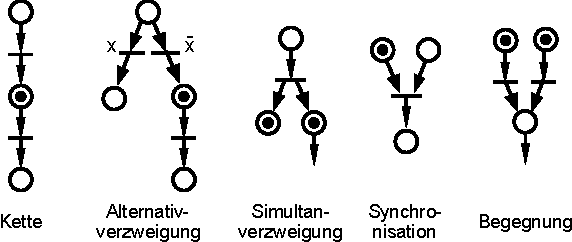
\includegraphics[width = \columnwidth]{./img/petri_constructs.pdf}

}


% SECTION ======================================================================
\section{Technik}
% ==============================================================================
\Fbox{${}^{\text{Bediener}}_{\text{Beobachter}}$} $\rightleftarrows$ \Fbox{${\text{Regler }}^{\ra \text{ Stellen}}_{\leftarrow \text{ Messen}}$} $\rightleftarrows$ \Fbox{Strecke}\\

\vspace{0.5cm}
Auch wichtig:

Schrödingers Katze: \parbox{1cm}{ 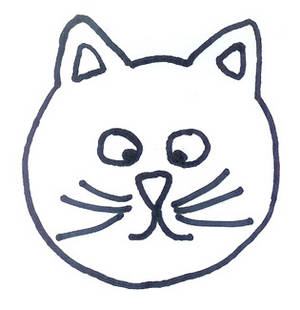
\includegraphics[width=1cm]{img/cat.jpg}}
% TODO: DGL System und resultierender Signalflussplan

\newpage

{\Huge \bf Anhang}

\subsection{Mögliche Arten von WOKs:}
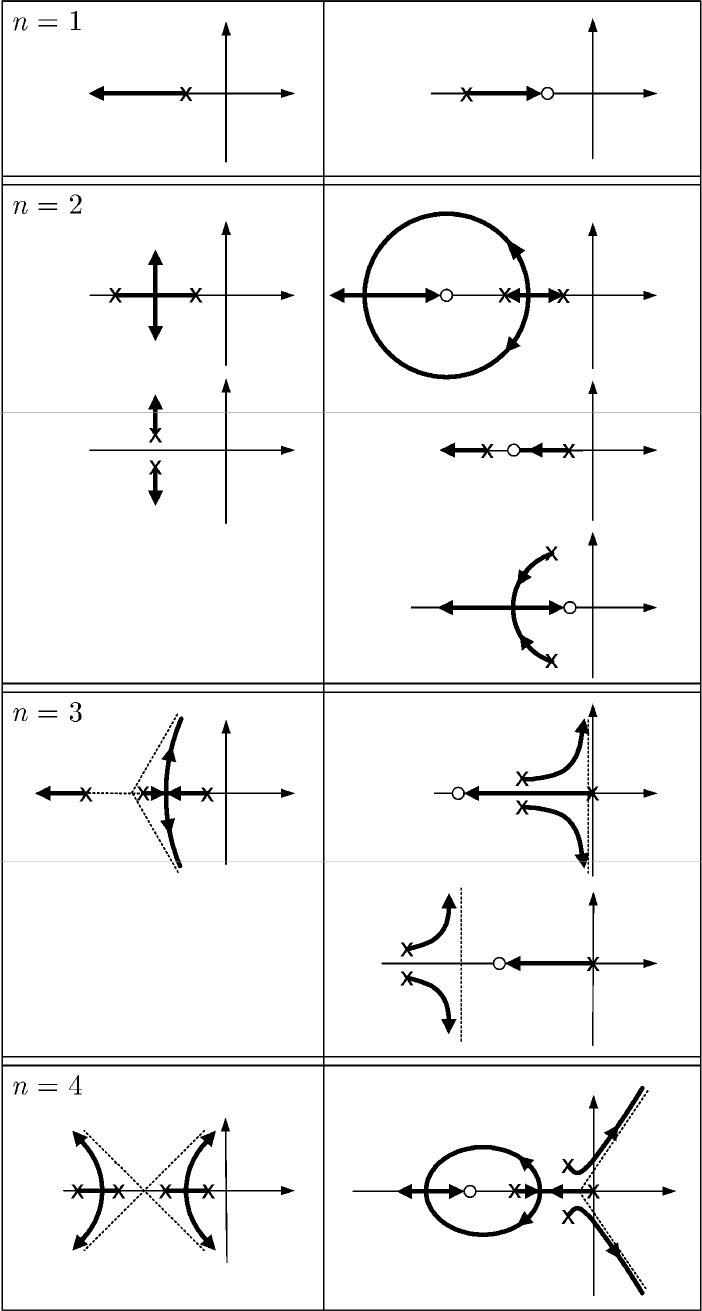
\includegraphics[width = \columnwidth]{./img/wok_kinds.jpg}

\columnbreak

\subsection{Normalformen}
\textbf{Kanonische Normalform:}\\
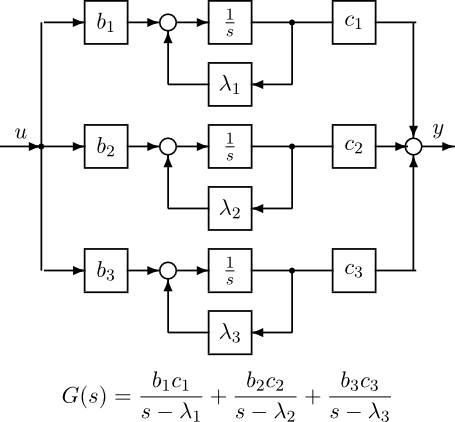
\includegraphics[width = 6cm]{./img/kanonischenormalform.jpg}\\
\textbf{Regelungsnormalformnormalform:}\\
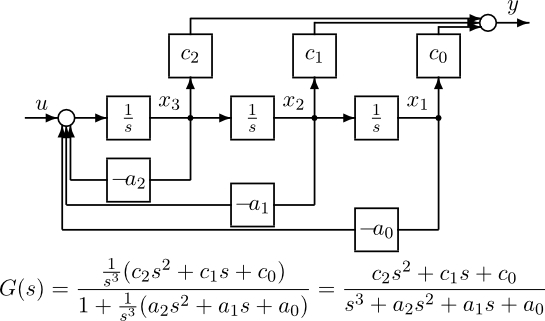
\includegraphics[width = 6.5cm]{./img/regelnormalform.jpg}\\
\textbf{Beobachtungsormalform:}\\
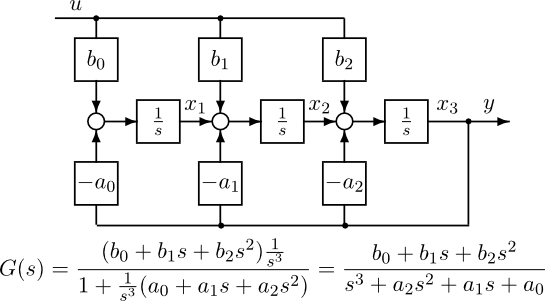
\includegraphics[width = 6.5cm]{./img/beobachternormalform.jpg}

\columnbreak


\subsection{Strecke/Regler Auswahl}
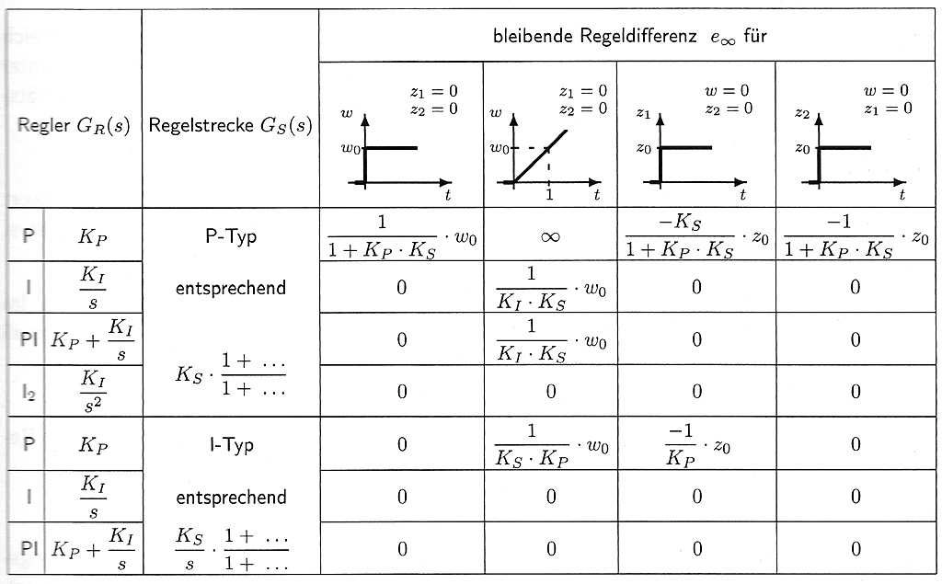
\includegraphics[width = 14cm]{./img/reglerstrecke.pdf}


\subsection{Zustandsbeobachter(Simulation)}
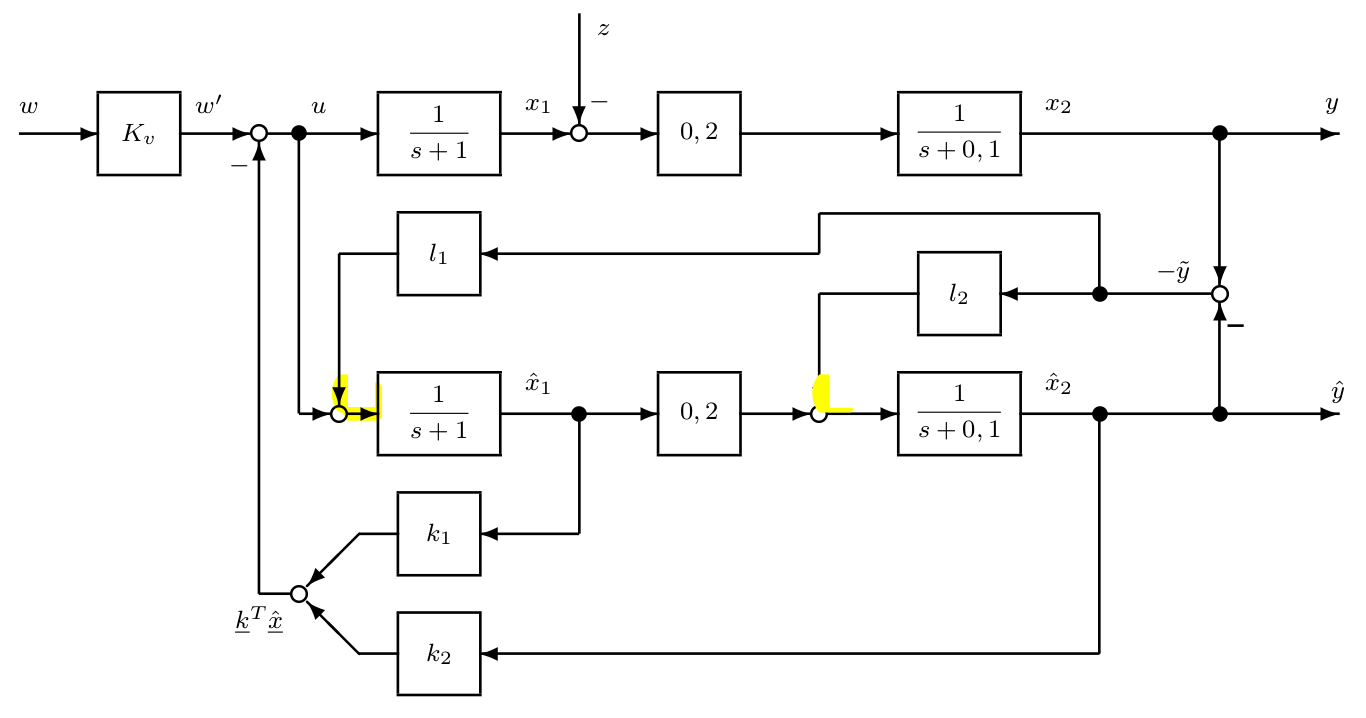
\includegraphics[width = 14cm]{./img/beobachter.jpg}


% Ende der Spalten
\end{multicols*}


% ###############################
\end{document}
% ###############################





\newpage

% Split in 2 Columns ===========================================================
\begin{multicols*}{2}


\begin{tabular*}{\columnwidth}{@{\extracolsep\fill}llll@{}} \ctrule
			& DGL & $G(s)$ & Sprungantwort $g(t)$\\
\textbf{P} & $y(t) = K_{\ir P} u(t)$ & $G(s) = K_{\ir P}$ & 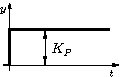
\includegraphics{./img/blocks/P_G.pdf}\\
\textbf{I} & $\dot y(t) = K_{\ir I} u(t)$ & $G(s) = \frac{K_{\ir I}}{s}$ \\
\textbf{D} & $y(t) = K_{\ir D} \dot u(t)$ & $G(s) = K_{\ir D} s$ \\
\textbf{T}$_t$ & \\


\textbf{PID} & \\
\textbf{PIDT}$_1$ & \\
\end{tabular*}






\end{multicols*}

% Midterm: Anfangs und Endwertsatz wichtig!

% Dokumentende
% ======================================================================
\end{document}

% ToDos:
